%!TEX root = ../thesis.tex
%*******************************************************************************
%****************************** Evaluation Chapter *********************************
%*******************************************************************************

\chapter{Evaluation}
\label{chap:evaluation}
In the previous chapter, we explained the implementation of our tool. 
Based on that, in this chapter, we will discuss the details of the evaluation process, including the user case study (see section \ref{evaluation:section:casestudy}), experimental design (see section \ref{evaluation:section:design}), execution (see section \ref{evaluation:section:execution}), analysis (see section \ref{evaluation:section:analysis}), and interpretation (see section \ref{evaluation:section:interpretation}) of the results. 
For the setup, we recruited participants from Paderborn University.
\ifpdf
    \graphicspath{{Chapters/Evaluation/Figs/}{Chapters/Evaluation/Figs/}{Chapters/Evaluation/Figs/}}
\else
    \graphicspath{{Chapters/Evaluation/Figs/}{Chapters/Evaluation/Figs/}}
\fi

\section{User Case Study}
\label{evaluation:section:casestudy}
To evaluate the effectiveness of our approach, we conducted a case study that involved recruiting participants, developing prototypes, and working on user scenarios. 
We recruited 15 participants who are students at Paderborn University. 
The case study is based on the evaluation stage of the first cycle of our DSR (as discussed in section \ref{introduction:section:research}). 
In conducting and reporting our case study research, we followed the established guidelines of Runeson and Höst \cite{eval:guidlines:runeson} (see figure \ref{evaluation:fig:casestudy}) to increase the quality of the study outcomes. 
These guidelines helped ensure our research was rigorous, transparent, and credible. 
By adhering to these guidelines, we aimed to provide a detailed and comprehensive account of our case study, enabling others to replicate our research and build upon our findings.
This case study also aims to develop the RQ as explained in the next section.

\clearpage
\section{Experimental Design}
\label{evaluation:section:design}
In this section, as per Runeson and Höst, we first define the objective, case study, research questions, and the methods we follow to complete the evaluation.

\paragraph{Objective:}
The objective of the user case study was to evaluate a \ac{poc} tool for creating and testing UI designs. 
The goal was to assess the tool's ability to generate UI prototypes, create split or A/B tests, and collect participant feedback to select the best variant.

\paragraph{Case Study:}
The case study involved a user scenario where John, a UX designer, was responsible for designing the UI for a new movie-streaming app. John used the \ac{poc} tool to create UI prototypes and perform split tests to select the best variant.

\paragraph{Research Questions (RQs):}
For the case study, we defined a couple of research questions. \\
\textbf{RQ1:} Can a \ac{poc} tool be used to prototype the UI of a new movie-streaming app and create split or A/B tests to select the best variant of the app's interface design? \\
\textbf{RQ2:} What feedback can be gathered from participants to evaluate the effectiveness of different app interface design variants?

\begin{figure}[ht]
    \centering
    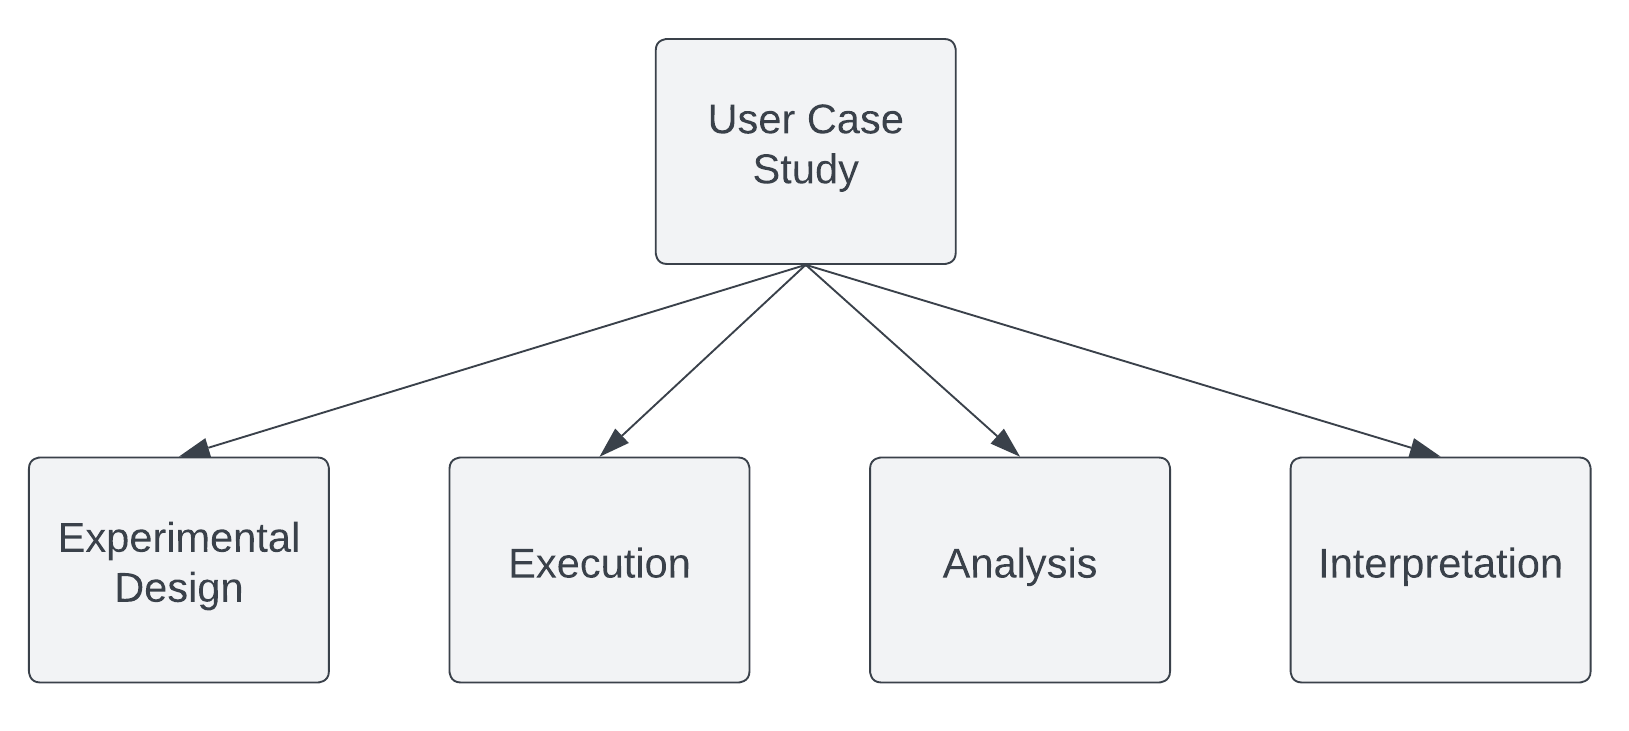
\includegraphics[scale=0.25]{case-study.png}
    \caption{User Case Study for Analysis}
    \label{evaluation:fig:casestudy}
\end{figure}

\paragraph{Method:}
For the User Case Study, we aimed to recruit diverse participants from different courses enrolled at Paderborn University to ensure a wide range of perspectives and experiences on UI prototyping and UI Experimentation. 
We wanted to include individuals with varying levels of experience in prototyping and user scenario development, from beginners to experts. 
To recruit participants, we used Doodle\footnote{Website for Doodle: \url{https://doodle.com/}}, an online tool for setting up the appointment, and a Line survey\footnote{Website for the survey: \url{https://umfragen.uni-paderborn.de/admin/}} hosted by our university for creating the questionnaire.

We developed a user scenario that required participants to use our UI prototyping tool hosted on the Paderborn University server. 
Therefore to access our tool, the participants needed to turn on the VPN\footnote{Website for University Paderborn VPN config: \url{https://imt.uni-paderborn.de/vpn-zugang/}} provided by the University. 
We also examined them using an open BigBlueButton\footnote{Website for BBB: \url{https://open-bbb.uni-paderborn.de/}} video conference session. 
We also considered the ethical clarifications by informing the participants that we were not recording the video conference session and that the survey was anonymous to ensure their privacy and encourage honest feedback while mentioning our data collection and storage strategy.

After using the tool, participants were asked to answer a questionnaire in the survey to provide qualitative and quantitative feedback for our tool and the \ac{dp}s we developed. 
The questionnaire was designed to evaluate the usability, effectiveness, and overall satisfaction with our tool. 
We also asked for suggestions for improvement and gathered additional comments and feedback from the participants to gain a deeper understanding of their experiences.

\clearpage
\section{Execution}
\label{evaluation:section:execution}
In this section, we explain the execution of our user case study in detail. 
First, we explain the planning phase of the execution and then explain the methodology of how we conducted the survey.

\paragraph{Planning:}
Before conducting the user case study, we carefully planned the experimental design to ensure the validity and reliability of our results.
First, we defined a hypothesis to be tested. We wanted our POC tool to fulfill the Design principles and validate the DPs. 
To achieve this, we developed a user scenario that involved the participants using our tool to create a prototype and conduct a user scenario. 
We recruited diverse participants enrolled in various courses at Paderborn University, with varying experience in prototyping and user scenario development.
To recruit participants for our case study, we shared a Doodle link via different communication channels, such as email and social media. 
The Doodle link contained the necessary information about the study, including the purpose, duration, and requirements. 
It also offered different time slots for the participants, ensuring that the survey could accommodate a diverse group of participants with varying schedules. 
This method helped us efficiently reach out to potential participants and allowed them to select a time that suited them best.

Secondly, we used the Lime survey, hosted on the Paderborn University server, to conduct a survey questionnaire to collect qualitative and quantitative feedback from the participants. 
The questionnaire was divided into three sections. 
The first section contained the \ac{sus} questionnaire, a widely used and reliable tool for measuring the usability of software systems. 
This section aimed to collect quantitative feedback from the participants regarding the usability of our prototype tool. 
The second section contained questions about the design principles we proposed in our thesis. 
This section aimed to collect participants' ratings and opinions on the effectiveness and feasibility of the design principles. 
The third section contained open-ended questions to gather participants' qualitative feedback and suggestions for improving our prototype tool and the \ac{dp}s. 
We used the Lime survey to facilitate the data collection process and to ensure anonymity and privacy for the participants.

\paragraph{Methodology:}
The methodology of our user case study involved using a proof of concept tool accessible via UPB VPN that combined qualitative and quantitative data collection and analysis techniques. The participants were then asked to conduct a user scenario using our tool while being observed through an open BBB video conference session.
The scenario was that John, a UX designer, was creating a new movie-streaming app and wanted to prototype different UI designs and conduct split tests to select the best variant. 
The study was conducted in several phases.

In the first phase, John explored the tool and generated an example movie streaming prototype using the headstart button. He then added new movies to the prototype using the data model feature.
In the second phase, John created split tests for different app interface versions. 
He used the tool's A/B testing feature to create two versions of the app's view screen and changed the UI to make some changes in the variant's prototype.
In the third phase, John created tasks for participants to complete and gather feedback on the app's interface. 
He also created a set of questionnaires, including open-ended and scale-based questions, to collect qualitative data from participants.
In the fourth phase, John recruited participants or used dummy users generated from the tool to test the experiments and monitor the results. 
After completing the experiment, John navigated to the experiments page and analyzed the statistics to determine which version of the app's interface was more effective.
Based on the feedback from the usability tests and questionnaires, John iterated on the app's design and updated the prototype in the tool. 
Overall, the execution of the experiment involved prototyping, split testing, task creation, and feedback gathering to design and improve the movie-streaming app's interface. 
An example prototype, created by one of the user participants is shown in Appendix \ref{appendix:three:caseStudy}.

\clearpage
\section{Analysis}
\label{evaluation:section:analysis}
After collecting the data through LimeSurvey and the tool, we analyzed the feedback and results to draw insights and conclusions about the effectiveness of our research questions and the software tool we designed. 
We also examined the qualitative feedback from the participants to gain a deeper understanding of their preferences and needs. 
Next, we explain the qualitative and quantitative analysis of the data collected from the participants in detail.

\paragraph{Quantitative analysis}
\begin{figure}[ht]
    \centering
    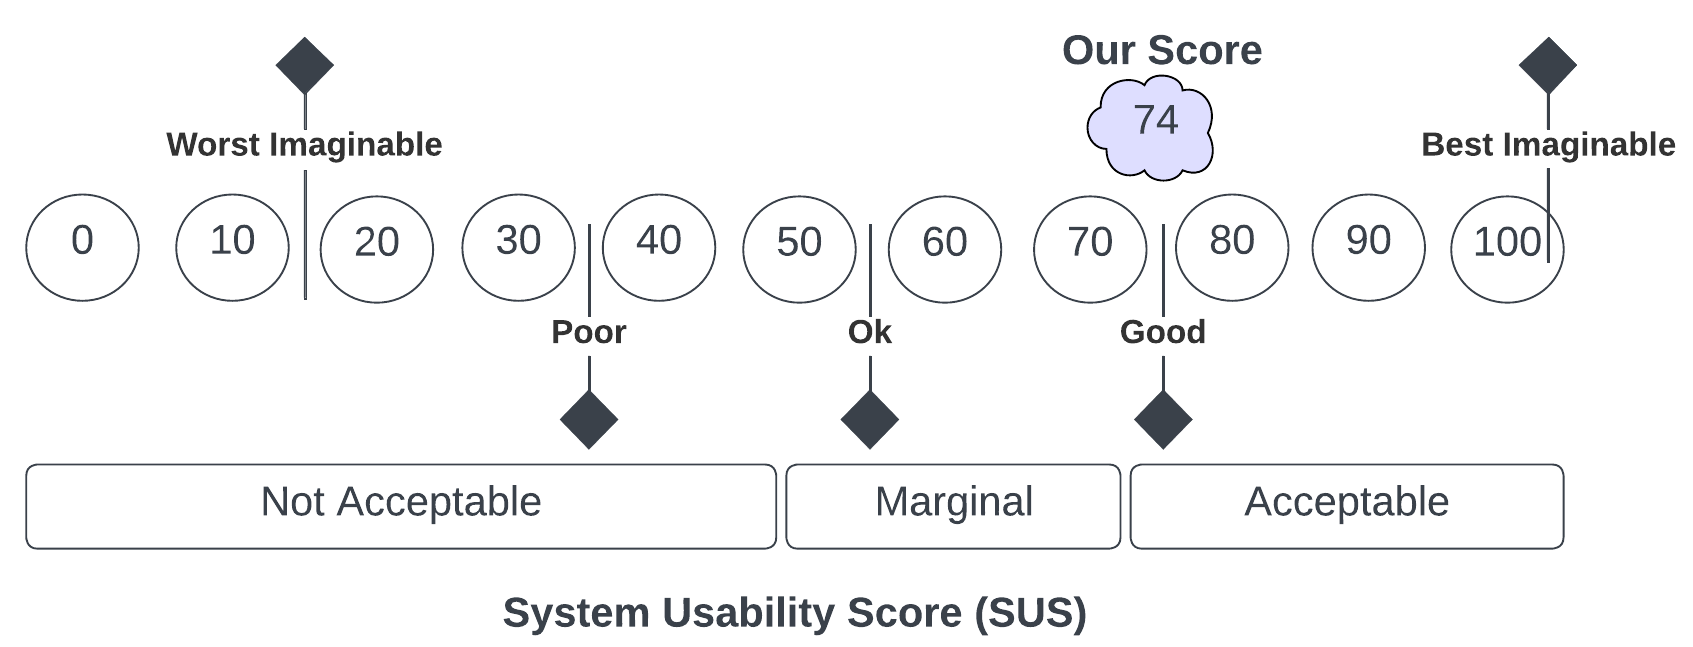
\includegraphics[scale=0.25]{SUS.png}
    \caption{System Usability score (SUS) of our tool}
    \label{evaluation:fig:sus}
\end{figure}
In the first part of the quantitative section of our analysis, we utilized the \ac{sus} to gather feedback on the usability of our tool. 
The \ac{sus} is a widely used and well-established questionnaire for assessing the usability of a system. 
It consists of 10 statements that participants rate on a 5-point scale from 1 (strongly disagree) to 5 (strongly agree). 
The scores from each report are then combined and transformed to create a final \ac{sus} score ranging from 0 to 100.
After administering the \ac{sus} questionnaire to our participants, we computed the average score to obtain a quantitative measure of the usability of our tool. 
We also analyzed the individual scores for each statement to identify areas where the tool performed well and where improvements could be made. 
It allowed us to gain insights into the strengths and weaknesses of our tool from a quantitative perspective. 
It provided a basis for making data-driven decisions about improving the tool's usability. 
Our analysis of the \ac{sus} survey responses revealed an average score of \textit{74} (see figure \ref{evaluation:fig:sus}), indicating that the overall usability of the app prototype was rated as ``\textit{good}'' by the participants.
This score is above the average \ac{sus} score of 68, suggesting that the app prototype had a high level of usability.

The second part of our survey focused on rating the DPs of the solution tool using a 5-point scale. 
Participants were asked to rate their agreement with statements related to each DP. 
To analyze the data, we calculated the mean and standard deviation for each DP, as well as plotted a boxplot (see figure \ref{evaluation:fig:boxplot}) to visualize the distribution of responses. 
The boxplot showed that the majority of participants had a positive rating for all DPs, with some variability in the extent of agreement. 
Overall, the results indicated that the design principles were well-received by participants and can be considered strengths of the app's design.

\begin{figure}[ht]
    \centering
\begin{tikzpicture}
    \begin{axis}[
        boxplot/draw direction=y,
        enlarge y limits,
        xtick={1,2,3,4,5,6,7,8,9},
        xticklabel style = {align=center, font=\small},
        xticklabels={DP1, DP2, DP3, DP4, DP5, DP6, DP7, DP8, DP9},
    ]
    %   [
    %   xtick={1,2,3},
    %   xticklabels={DP1, DP2, DP3},
    %   ]
      \addplot+[draw=black, solid,
      boxplot prepared={
        median=5,
        upper quartile=5,
        lower quartile=4,
        upper whisker=5,
        lower whisker=3
      }, fill=lightgray
      ] coordinates {};
      \addplot+[draw=black, solid,
      boxplot prepared={
        median=5,
        upper quartile=5,
        lower quartile=4,
        upper whisker=5,
        lower whisker=3
      }, fill=lightgray
      ] coordinates {};
      \addplot+[draw=black, solid,
      boxplot prepared={
        median=4,
        upper quartile=5,
        lower quartile=4,
        upper whisker=5,
        lower whisker=2
      }, fill=lightgray
      ] coordinates {};
      \addplot+[draw=black, solid,
      boxplot prepared={
        median=4,
        upper quartile=5,
        lower quartile=4,
        upper whisker=5,
        lower whisker=4
      }, fill=lightgray
      ] coordinates {};
      \addplot+[draw=black, solid,
      boxplot prepared={
        median=4,
        upper quartile=4.5,
        lower quartile=3.5,
        upper whisker=5,
        lower whisker=2
      }, fill=lightgray
      ] coordinates {};
      \addplot+[draw=black, solid,
      boxplot prepared={
        median=4,
        upper quartile=5,
        lower quartile=4,
        upper whisker=5,
        lower whisker=3
      }, fill=lightgray
      ] coordinates {};
      \addplot+[draw=black, solid,
      boxplot prepared={
        median=4,
        upper quartile=4.5,
        lower quartile=4,
        upper whisker=5,
        lower whisker=1
      }, fill=lightgray
      ] coordinates {};
      \addplot+[draw=black, solid,
      boxplot prepared={
        median=4,
        upper quartile=5,
        lower quartile=4,
        upper whisker=5,
        lower whisker=3
      }, fill=lightgray
      ] coordinates {};
      \addplot+[mark=*, draw=black, solid,
      boxplot prepared={
        median=5,
        upper quartile=5,
        lower quartile=4,
        upper whisker=5,
        lower whisker=3
      }, fill=lightgray
      ] coordinates {};
    \end{axis}
  \end{tikzpicture}
  \caption{Box Plot analysis of the \ac{dp}s}
  \label{evaluation:fig:boxplot}
\end{figure}

\paragraph{Qualitative analysis}
For the qualitative analysis, we had three open-ended questions in the survey. 
The first question asked participants if they could complete their scenario efficiently using the software and, if not, what difficulties they encountered. 
Many participants noted that they could complete their scenario without any issues, while a few mentioned that they had trouble navigating the software or understanding how to use certain features.
The second question asked participants if there were any areas where the tool could be improved to meet their needs better. 
Several participants suggested adding more customization options for UI elements.
The third question asked participants if they would recommend this UI prototyping tool to others and why or why not. 
Many participants said they would recommend the tool, citing its ease of use and ability to create and test UI prototypes quickly. 
Some participants noted that the tool could be improved in certain areas but still felt it was valuable overall.

\clearpage
\section{Interpretation}
\label{evaluation:section:interpretation}
In this section, we interpret the feedback obtained from the user case study and analyze the quantitative and qualitative analysis. 
The feedback and user comments will be used to identify the areas where the tool can be improved to better meet the needs of its users. 
We will also discuss the lessons learned from the feedback and analysis and how they can be applied to future tool iterations. 
The insights gained from this section will be valuable in guiding the development and improvement of the tool to provide an optimal user experience for its users.

\paragraph{Quantitative data}
The \ac{sus} is a widely used measure of the perceived usability of a system. 
The average SUS score of 74 (see figure \ref{evaluation:fig:sus}) indicates that the users found the tool reasonably usable. 
However, the score could be higher, suggesting that there is still room for improvement. 
The \ac{sus} score provides a broad measure of overall usability but does not provide specific details on areas that may require improvement. 
Therefore, it is necessary to look at the individual user feedback and the box plots of the \ac{dp}s to identify areas that need improvement.

To further analyze, we looked at the individual DPs box plots (see figure \ref{evaluation:fig:boxplot}). 
Box plots are a way of graphically representing the distribution of data. 
The box represents the middle 50\% of the data, with the median value marked by a line in the box. 
The whiskers extend to the highest and lowest data points within 1.5 times the upper and lower quartiles' interquartile range (IQR). 
Any data points beyond the whiskers are marked as outliers.
Looking at the box plots for the DPs, we can see that DP1, DP2, DP6, DP8, and DP9 all have similar distributions with median scores of 4 or 5, upper quartiles of 5, and lower quartiles of 4. 
These DPs were generally well-received by users, with most participants rating them as good or excellent.
On the other hand, DP3, DP5, and DP7 have lower median scores of 4, indicating that users rated them as slightly less usable than the other DPs. 
DP3 and DP5 have wider distributions, with lower quartiles of 2 and 3.5, respectively, indicating that some users found them particularly challenging. 
DP7 has a particularly low lower quartile of 1, meaning that some users found it very difficult to use.
Overall, the box plot analysis suggests that some areas of the tool are particularly challenging for users, and these should be the focus of improvement efforts. 
Specifically, improvements to DP3, DP5, and DP7 could be prioritized to make them more usable and user-friendly in the next cycle or iterations of the \ac{dsr}.

\paragraph{Qualitative data}
Three open-ended questions were asked to the participants from the responses to the question \textit{Were there any areas where the tool could be improved to better meet your needs?}, we received 15 responses. 
A few respondents didn't have any specific suggestions (A$_1$ and A$_2$) (here \textit{A$_n$} means answer from nth participant). 
However, some participants recommended adding new features or enhancing the existing ones. 
For instance, A$_3$ suggested including the ability to configure whether users can go back in the questionnaire, editing, and reordering created tasks and questionnaires, and providing more data analysis options. 
A$_4$ proposed adding a more intuitive button to extend experiments or tasks. 
A$_5$ and A$_6$ recommended adding the ability to see how much space UI components take when creating views and improving the analysis graph's size and readability. 
A$_7$ suggested enhancing the tool's appearance to make it more attractive. 
A$_8$ recommended making the User Guide more intuitive and easier to follow, possibly with examples. 
A$_9$ suggested improving the aesthetics and reducing the complexity of certain features. 
A$_{10}$ recommended adding more variations for UI elements, such as drop-downs, and refining the result analysis to be more visually appealing. 
A$_{11}$ suggested several improvements, such as providing freedom to change the size of elements in a view, displaying the tasks in the testing view, and reducing the number of feedback confirmations during tasks.
A$_{12}$ suggested improving the data model and views sections' explanations.
A$_{13}$ recommended improving the image variable. 
A$_{14}$ and A$_{15}$ suggested providing clearer instructions to make the tool easier to use.

Based on these responses, the tool has several areas for improvement. 
Some participants suggested adding new features, while others recommended improving existing features' usability and aesthetics. 
Some of the most common suggestions included improving the appearance and usability of the tool, refining the result analysis, and providing more thorough explanations of features in the User Guide. 
The development team can use these suggestions to enhance the tool's functionality and make it more user-friendly for future users. 